\documentclass[11pt]{report}
\usepackage[T1]{fontenc}
\usepackage[french]{babel}
\usepackage[utf8]{inputenc}
\usepackage{graphicx}
\usepackage{caption}
\usepackage{amsmath}
\usepackage{amsfonts}

%Corps du document :
\begin{document}
\title{FCSR-h Filtrés}
\maketitle

    %Hello World \LaTeX{} !
    
\chapter{LFSR}
	\section{Définition}
	Un registre à décalage à rétroaction linéaire ou LFSR (Linear Feedback Shift Register) constitue en un élément de base des générateurs pseudo-aléatoires de génération de suites de chiffres.
	%saut	
	
	Un LFSR binaire de longueur $n$ est composé d'un bloc de $n$ bits appelé registre  ($a_0,...,a_n$) et d'une fonction de rétroaction linéaire.
	Cette fonction $f$ est de la forme : 
	\[
	f(a_0,a_1,...,a_n)=q_0a_0+q_1a_1+...+q_na_n
	\].
	
	\section{Architecture Fibonacci}
	Le registre est initialisé avec $r$ bits $(a_0,a_1,...,a_{r-1})$. A chaque cycle d'horloge ces bits sont additionnés (modulo 2) multipliés par les $q_i$ décrits plus hauts. \\Le bit résultant de cette opération : \\
	\[
	a_r = \sum_{i=0}^{r-1} a_iq_{r-i}\,(mod 2)
	\]
	va par la suite être réinjecté dans la première cellule. Les autres bits seront tous décalés vers la cellule de droite ($a_i => a_{i+1}$).
	\begin{figure}[!h]
	\centering
	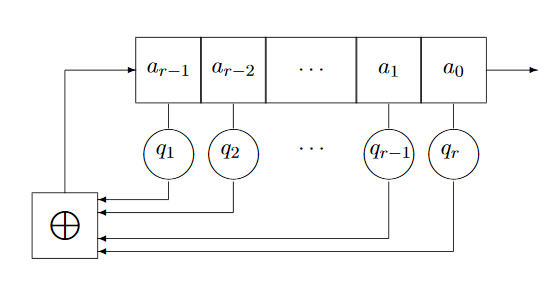
\includegraphics{FIBOLfsr.png}
	\caption{LFSR Architecture Fibonacci}
	\label{LFSRFibo}
	\end{figure}
	\\
	\\\\\\\\
	
	\textbf{Exemple:} LFSR à 4 bits avec $(q_0,q_1,q_2,q_3)=(1,1,0,1)$ 
	\begin{itemize}
	\item Initialisation du registre avec : $(0,1,1,0)=(a_3,a_2,a_1,a_0)$
	\item Premier tic : on calcule $a_4=0*q_0+1*q_1+1*q_2+1*q_3 = 1$ bit de sortie $a_0 = 0$. Nouvel état du registre : $(a_4,a_3,a_2,a_1)=(1,0,1,1)$
	\item Second tic d'horloge : $a_5=1*q_0+0*q_1+1*q_2+1*q_3$
	\item ...
	\item Au septième tic on retrouve l'état initial : $(0,1,1,0)$
	\end{itemize}
	
	
	
	
	\section{Architecture Galois}
	
	Dans la représentation Galois d'un LFSR les choses se présentent de la manière suivante : 
	Pour un LFSR de longueur r, à chaque tic d'horloge, chaque cellule $a_i$ est mise à jour avec le calcul : 
	\[
	\forall i \in {1,..,r-2}, 
	\,a_i = a_{i+1} + q_{i+1}a_0 \,(mod 2)\]
	\[ a_{r-1} = q_ra_0
	\]
	
	$a_{r-1}$ devient donc la première cellule du registre. 
	\\
	\begin{center}
	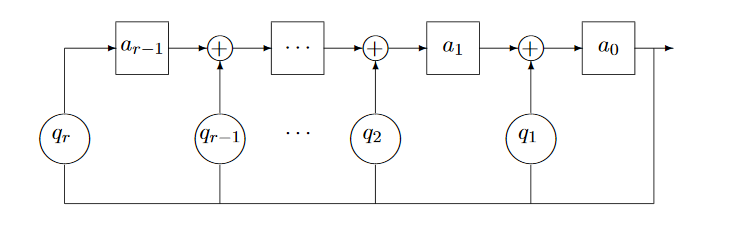
\includegraphics{GaloisLFSR.png}
	\captionof{figure}{LFSR Architecture Galois}
	\label{LFSRGalois}
	\end{center}
	
	A chaque LFSR de longueur r (dans les deux architectures), on associe le polynôme de rétroaction (ou caractéristique) suivant : 
	\[
		q(X) = q_rX^r + q_{r-1}X^{r-1} + ... + q_1X + 1
	\]	
	A noter qu'on appelle polynôme de connexion l'inverse du polynôme caractéristique : 
	\[
		b(X) = q(1/X)X^r
	\]
	
	
\chapter{FCSR}
\section{Définition}
Les FCSR (Feedback with Carry Shift Register) sont analogues aux LFSR en utilisant non plus l'addition modulo 2 mais dans $\mathbb{Z}$.
Un FCSR de longueur $r$ est construit de manière quasi identique à un LFSR : on dispose de $r$ cellules $(a_0,..,a_{r-1})$ et d'une nouvelle cellule $m$ servant de "retenue" (carry en anglais) à l'addition dans $\mathbb{Z}$.

\section{Architecture Fibonacci}
A la manière des FCSR en architecture Fibonacci, à chaque tic d'horloge, on calcule une somme $z$ intermédiaire, puis on va décaler à droite l'ensemble des cellules du registre. A la différence que cette fois-ci on va garder la retenue et le contenu de la première cellule est le bit de parité de la somme.  
\\
Cela se présente comme tel : 
\\
On somme : 
\[
z= m + \sum_{i=0}^{r-1} a_iq_{r-i} \in \mathbb{Z}
\]
\\
On décale à droite l'ensemble des cellules : 
$a_i = a_{i+1},\; \forall i \in [0,..,r-2]$
\\
La première cellule $a_{r-1}$ prend la valeur du bit de parité $(z \,mod(2))$. 
\\
La nouvelle cellule de "retenue" $m$ prends la valeur des autres bits de $z$ : 
\[
 	m = z\, div \,2 \;\; \textnormal{(le quotient de la division euclidienne de z par 2)}
\]

\begin{center}
	
	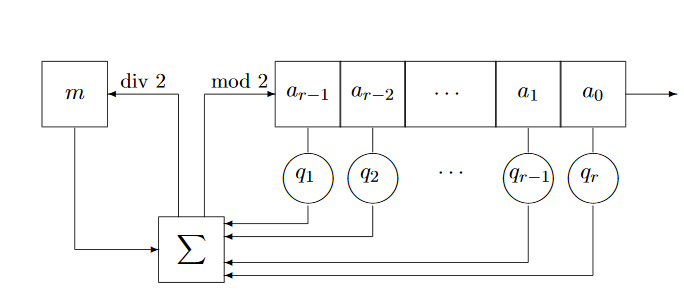
\includegraphics[scale=0.7]{FiboFCSR.png}
	\captionof{figure}{FCSR Architecture Fibonacci}
	\label{FCSRFibo}

\end{center}

\section{Architecture Galois}
	
	Concernant les FCSR en mode Galois, à l'instar de l'architecture Fibonacci, on retrouve des similitudes aux LFSR Galois. Le bit $a_0$ sert également de rétroaction à tous les autres. Les additions sont cette fois faites avec "retenue", et cette donnée est stockée dans une nouvelle cellule $c_i$ relative à sa cellule $a_i$.
	\\
	A chaque tic d'horloge un FCSR de longueur $r$ est mis à jour de la façon suivante : 
	$$	
	\forall i \in \{0,...,r-1\},
	 \left\{
	 \begin{array}{ccc}
	 z_i = a_{i+1} + c_i + q_{i+1}a_0\\
	 a_i = z_i \, mod \,2\\
	 c_i = z_i \, div \,2\\
	 \end{array} 
	\right. 
	$$
	
	Finalement, la première cellule devient : $a_{r-1}=c_{r-1}+q_ra_0$
	
	\begin{center}
	
	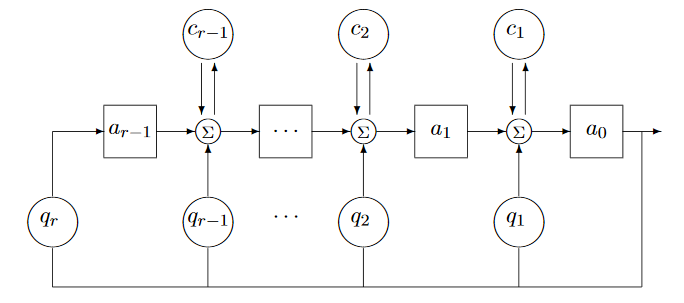
\includegraphics[scale=0.7]{GaloisFCSR.png}
	\captionof{figure}{FCSR Architecture Fibonacci}
	\label{FCSRGalois}
	\end{center}
	
	Le $\Sigma$ représente les $z_i$ intermédiaires.
	\\\\
\textbf{Remarque :} on aurait pu introduire la notion de temps $t$ à nos cellules du registre. C'est cependant totalement équivalent au modèle présenté dans les chapitres précédents : $(a_0(t) \Leftrightarrow a_{0+t})$ cela simplifie la compréhension pour la suite. \\\\

	Dans les deux architectures on peut associer un FCSR de longueur r à un "entier de connexion" : 
	$$
	q = q_r2^r + q_{r-1}2^{r-1} + ... + q_12 - 1 \in 
	\mathbb{Z}
	$$
	Pour la suite on pose $d = (1+|q|)/2$ dans certains articles cet entier est préféré pour considérer les calculs.
	\\\\
	Considérant le temps $t$ on peut introduire les formules suivantes pour simplifier les calculs et décrire la fonction de transition: 
	\begin{align*}
		a_i(t+1) &= a_{i+1}(t) \, div \, 2 \oplus d_ic_i(t) \oplus d_ia_o(t)\\
		c_i(t+1) &= a_{i+1}(t)c_i(t) \oplus c_i(t)a_0(t) \oplus a_o(t)a_{i+1}(t)
	\end{align*}
		
	
	\section{Entiers 2-adiques}
	
	Un entier 2-adique est une série formelle $\alpha = \sum_{i=0}^\infty a_i2^i$ avec $a_i \in \{0,1\}$.
	Ces séries ne convergent pas à proprement parler (elles convergent au sens de la topologie 2-adique) mais peuvent être tout de même manipulées en le considérant. L'ensemble de telles séries forme l'anneau $\mathbb{Z}_2$ des entiers 2-adiques. La différence entre cet anneau et l'anneau $\mathbb{Z}/2\mathbb{Z}[X]$ est que l'addition dans $\mathbb{Z}_2$ est réalisée en reportant les retenues sur les termes d'ordre supérieur, $i.e\;\forall n \in \mathbb{N},\quad 2^n+2^n = 2 \cdot 2^n = 2^{n+1}$.
	\\
	S'il existe un entier $N$ tel que $a_n=0 \; \forall \, n \geq N$ alors $\alpha$ est un entier positif. Chaque entier impair $q$ a un inverse dans $\mathbb{Z}_2$
	\\
	\\
	\textbf{Proposition:} Soit $A=(a_n)_{n \in \mathbb{N}}$ une séquence binaire et $\alpha = \sum_{i=0}^\infty a_i2^i$ l'entier 2-adique correspondant. La séquence $A$ est ultimement périodique si et seulement si, il existe deux nombres $p$ et $q$ (avec $q$ impair $\iff q=1\,mod2$)  dans $\mathbb{Z}$ tel que $\alpha = p/q$. De plus $A$ est strictement périodique si $pq \leq 0$ et $|p| \leq |q| \;(\iff |\alpha| \leq 1)$.
	\\
	\\
	La période de $A$ est l'ordre de 2 modulo $q$ (i.e le plus petit entier $T$ tel que $2^T = 1\,mod \,q$). Si $q$ est premier alors $T$ est un diviseur de $|q| - 1$. 
	\\
	A partir de la proposition précédente on peut définir un FCSR à l'aide d'un entier $q$ premier et d'une valeur initiale $p$.
	
	\section{Conséquences sur les FCSR}
	\subsection{Mode Fibonacci}
	Dans cette section on considère un FCSR de longueur r en architecture Fibonacci avec un entier de connexion $q$ comme décrit plus haut, une retenue initiale $m_{r-1}$ et un registre initial $(a_0,...,a_{r-1}$ 
	\\
	Ce registre va donc générer une séquence infinie, potentiellement périodique, $A = (a_0,a_1,a_2,...)$ de bits associée à son entier 2-adique $\alpha = \sum_{i=0}^\infty a_i \cdot 2^i$.
	On a $q = \sum_{i=0}^r q_i \cdot 2^i$ avec $q_0 = -1$, on définit : 
	\[
	p= \sum_{i=0}^{r-1} \sum_{j=0}^i q_ja_{i-j}2^i - m_{r-1}2^r
	\]
	\\
	\\
	\textbf{Théorème:}
	La sortie $A$ d'un FCSR comme définit plus haut est la séquence de bits de la représentation 2-adique du nombre rationnel $\alpha = p/q$, soit :
	\[
	\alpha = \sum_{i=0}^\infty a_i \cdot 2^i = p/q \in \, \mathbb{Z}_2
	\]	
	
	On comprend donc que pour un même FCSR, différents état initiaux vont donner des séquences radicalement distinctes. 
	\\
	\\
	\textbf{Corollaire:}
	Soit $A=(a_0,a_1,a_2,...)$ une séquence potentiellement périodique, alors son entier 2-adique associé $\alpha = \sum a_i \cdot 2^i$ est le quotient de deux entiers $p$ et $q$ (le quotient $p/q$ est un nombre rationnel). Le dénominateur $q$ est l'entier de connexion qui génère la séquence $A$. Cette séquence est strictement périodique si et seulement si $p \leq 0$ et $|\alpha| \leq 1$.
	\\
	\\
	\textbf{Preuve du théorème:}
	Dans cette preuve, on considère les calculs dans $\mathbb{Z}_2$. Regardons la transition d'un état du FCSR en architecture Fibonacci, en supposant $n$ transitions au préalable. En posant la longueur $r \in \mathbb{N}$ On a donc, une valeur de retenue $m_{n-1}$ et le contenu du registre étant les $r$ bits $(a_{n-1},a_{n-2},...,a_{n-r})$ explicités précédemment (on a $a_{n-1}$ la dernière "nouvelle" cellule, la plus à gauche, et $a_{n-r}$ la dernière cellule du registre, la plus à droite, sachant que le registre se décale vers la droite). 
	\\
	Afin d'effectuer la transition vers le nouvel état, on procède comme expliqué, on somme : 
	
	\[
		z_n = m_{n-1} + \sum_{i=1}^{r} a_iq_{n-i}
	\]
On remplace le contenu de la cellule de retenue : $$m_n = z_n\, div\, 2$$
On décale tous les bits vers la droite, et la nouvelle cellule la plus à gauche devient : 
$$a_n = z_n \, mod \, 2$$
\\
Ces équations peuvent être combinées en une seule :
$$z_n = 2m_n + a_n$$
Ce qui implique : 
$$a_n = \sum_{i=1}^r q_{n-i} \cdot a_i+(m_{n-1}-2m_n)$$

On a les valeurs initiales du FCSR représentées par : $(a_0,a_1,...,a_{r-1})$ (valeurs des bits) et $m_{r-1}$ (cellule de retenue). 
Si on reprend l'équation du théorème pour $\alpha$ cela donne :
\begin{align*}
\alpha &= \sum_{i=0}^\infty a_i \cdot 2^i\\
	&=	a_0 + a_12 + \cdots + a_{r-1}2^{r-1} + 		\sum_{n=r}^\infty a_n2^n\\
	&= x + \sum_{n=r}^\infty(\sum_{i=1}^r q_{n-i}a_i) \cdot 2^n \, + \sum_{n=r}^\infty (m_{n-1} - 2m_n)2^n\\
\end{align*}



Où :
$$ x = a_0 + 2a_1 + 2^2a_2 + \cdots + a_{r-1}2^{r-1} $$
l'entier représentant la valeur initiale des cellules du registre.
\\
\\
\textbf{Remarque:}
$$
\sum_{i=1}^r q_{n-i}a_i \Leftrightarrow \sum_{i=1}^r q_ia_{n-i}
$$
Cela peut servir pour certains calculs 
\\
\\
La seconde sommation dans l'équation de $\alpha$ s'annule à l'exception du premier terme $m_{r-1}$, ce qui donne : 
\begin{align*}
\alpha &= x + m_{r-1}2^r + \sum_{n=r}^\infty\sum_{i=1}^r q_i2^ia_{n-i}2^{n-i}\\
&= x + m_{r-1}2^r + \sum_{i=1}^r q_i2^i(\sum_{n=r}^\infty a_{n-i}2^{n-i})\\
&= x + m_{r-1}2^r + \sum_{i=1}^r q_i2^i(\alpha - (a_02^0+a_12^1 + \cdots + a_{r-i-1}2^{r-i-1}))\\
&= x + m_{r-1}2^r + \alpha \cdot \sum_{i=1}^r q_i2^i - \sum_{i=1}^{r-1}\sum_{j=0}^{r-i-1} q_i \cdot 2^i \cdot a_j \cdot 2^j\\
\end{align*}

La somme du milieu étant nulle quand $i=r$ ce qui nous ramène à :

\begin{align*}
\alpha &= \frac{x + m_{r-1}2^r - \sum_{i=1}^{r-1}\sum_{j=0}^{r-i-1} q_i \cdot 2^i \cdot a_j \cdot 2^j }{1 - \sum_{i=1}^r q_i2^i}\\
&= \frac{\sum_{i=0}^{r-1}\sum_{j=0}^{r-i-1} q_i \cdot a_j \cdot 2^{i+j} - m_{r-1}2^r}{q}
\end{align*}
On opère un changement de variable avec $k = i+j$
ce qui nous donne :
$$
\alpha = \frac{\sum_{k=0}^{r-1}\sum_{i=0}^k q_ia_{k-i}2^k - m_{r-1}2^r}{q} = \frac{p}{q} 
$$
\begin{flushright}
$\square$
\end{flushright}

\subsection{mode Galois}
On sait que comme les LFSR, les deux architectures de FCSR sont équivalentes, et dans le cas de celle dite de Galois les choses se présentent comme telles : 
\\
Pour un FCSR en mode Galois de longueur $r$ de registre initial $(a_0,a_1, ... , a_{r-1})$ de cellules de retenues initiales $(c_1,c_2, ...,c_{r-1})$, on rappelle que l'entier de connexion est définit par :
$$
q = -1 + q_12^1 + \cdots + q_{r-1}2^{r-1} + q_r2^r
$$
 on définit le $p$ présenté plus haut par : 
$$
p= a_0 + (a_1 + c_1)2 + \cdots + (a_{r-1} + c_{r-1})2^{r-1}
$$
\\
Le théorème vu précédemment s'applique de la même façon, pour un tel FCSR la séquence qu'il produit est la séquence de coefficients de l'expansion 2-adique du nombre rationnel $\alpha = \frac{p}{q}$.

\subsection{Paramètres d'un FCSR}

On rappelle qu'un FCSR produit la représentation 2-adique du nombre rationnel $p/q$. Pour le construire $p$ dépend de la clé secrète et du IV (Initial Vector) comme nous l'avons vu précédemment, mais $q$ est un paramètre public, et il détermine la période. Il est important que $q$ remplisse certaines conditions. $q$ doit être un nombre premier impair (négatif selon les représentations) avec $log_2(q)=n+1$. L'ordre de 2 modulo $q$ est $|q| - 1$ et $T=(|q|-1/2)$ la période, est également un nombre premier. 


\chapter{Filtres sur les FCSR}

\section{Introduction}
	
	Dans les chapitres précédents, nous avons présenté des générateurs de nombres pseudo-aléatoires classiques se basant sur des objets mathématiques avancés. Les propriétés des FCSR sont bien connues: hautement non-linéaires, périodiques et présentent de très bonnes dispositions statistiques. Mais cela n'est pas suffisant, en effet étant donné la suite générée, on peut toujours reconstruire le modèle de base (entier de connexion par exemple), il n'y a rien de proprement secret.  Dans le cas des automates LFSR, dans le but de reconstruire le modèle, on peut par exemple citer l'algorithme de Berlekamp-Massey. On utilisera un algorithme analogue à ce dernier dans le cas des FCSR. 
	\\
	\\	
	C'est pour cette raison que l'idée d'introduire des filtres sur les cellules des FCSR est apparu. Grâce à la non-linéarité de tels automates, le meilleur filtre est simplement un filtre linéaire, qui effectue un XOR ("ou exclusif" équivalent à une additions de bits modulo 2) sur certains états du registre. On appelle cela les FCSR filtrés (Filtered FCSR, ou encore F-FCSR). 

\section{Reconstruction du modèle des FCSR}

	Dans cette section, nous allons montrer un algorithme permettant de retrouver les entiers relatifs $p$ et $q$ (bases du modèle des FCSR). 
	 \\
	 L'algorithme que nous allons présenter est analogue à l'algorithme de Berkelamp-Massey qui lui, résout le problème de reconstruction du modèle des LFSR. \\
	 On considère que l'on a une séquence binaire $a = (a_0,a_1,..)$ potentiellement périodique. On pose également $\phi$ la fonction telle que:\\
	 $\forall \; f=(f_1,f_2) \; \in \; \mathbb{Z} \times \mathbb{Z},$\\
	 $$\phi(f)=max(|f1|,|f2|)$$
	 
	 \textbf{Algorithme :} \\\\
	 Début : \\\\
	 Entrer les $a_i$ jusqu'à rencontrer le premier $a_{k-1}$ non nul\\
	 $\alpha = a_{k-1} \cdot 2^{k-1}$\\
	 $f \; = \; (0,2)$\\
	 $g \; = \; (2^k-1,1)=(g_1,g_2)$\\\\
	 \textbf{Tant que} il reste des bits \textbf{Faire:}\\
 entrer un nouveau bit $a_k$ \\ 
 $\alpha = \alpha + a_k2^k$\\
 \textbf{Si} $\alpha \cdot g_2 - g_1 \equiv 0 \pmod(2^{k+1})$ \textbf{alors:}\\ 
 $f = 2 \cdot f$\\
 \textbf{Sinon si} $\phi(g) < \phi(f)$ \textbf{alors:}\\
 $d = min(\phi(f+d \cdot g))$\\
 ($d \equiv 1 \pmod 2$)	 \\
 $(g,f)=(f+d \cdot g, 2g)$\\
 \textbf{Sinon:}\\
 $d = min(\phi(g+d \cdot f))$\\
 ($d \equiv 1 \pmod 2$)	 \\
  $(g,f)=(g+d \cdot f, 2f)$\\\\
  $k=k+1$\\
  \textbf{Retourner} $g$\\
 
\section{F-FCSR}

\textbf{Question : comment filtrer un automate FCSR?}\\
Dans le cas des LFSR de nombreux outils ont été utilisés dans le but de masquer la structure du générateur, notamment en utilisant des fonctions booléennes avec des propriétés précises afin de combiner plusieurs LFSR, utilisant des combineurs avec mémoire, ou en réduisant la séquence produite par les LFSR.\\
Il est possible d'utiliser des méthodes similaires dans le cas des FCSR, mais il n'est pas nécessaire d'utiliser des fonctions de filtrage hautement non linéaires. 
\\
On introduit les fonctions linéaires de filtrage de FCSR : 
$
f: \mathbb{F}_2^n \rightarrow \mathbb{F}_2,
$
$$
f(x_1,x_2,...,x_n) = \oplus_{i=1}^n f_ix_i, \; f_i \; \in \mathbb{F}_2
$$
Avec $\oplus$ la somme directe dans le corps $\mathbb{F}_2$.
\\\\
Grâce à cette fonction de filtrage, on filtre les $k$ cellules $a_i(t)$ du registre principal, on ne s'occupe pas des cellules de retenue. Afin de modéliser la séquence de notre FCSR filtré (à 1 filtre), on considère le vecteur binaire $F=(f_0,f_1,...,f_{k-1})$ de longueur $k$. La séquence produite par ce FCSR est donc :
$$
S=(s(t))_{t \in \mathbb{N}},
$$
où
$$
s(t) = \oplus_{i=1}^k f_i \cdot a_i(t)
$$

\section{F-FCSR-H}

Concernant le F-FCSR-H, le nombre de bits extraits est désormais 8. On considère donc maintenant 8 vecteurs linéaires $F_0,F_1,...,F_7$. Par contre, le vecteur linéaire $F_j$ ne considère que les cellules $a_i$ du registre avec $i$ satisfaisant $i \equiv j \pmod 8$. On va donc non plus produire des bits mais des octets. \\
En paramètres, on utilise une clé de longueur 80 et un vecteur initial (IV) de longueur binaire $v$ avec $32 \leq v \leq 80$. La taille du FCSR (le nombre de cellules du registres) est $n=160$. Et les cellules de retenue sont au nombre de $l = 82$.
\\
On pose
$$
q=1993524591318275015328041611344215036460140087963$$
ce qui nous donne : 
$$
d=(1+|q|)/2 = (AE985DFF\; 26619FC5\; 8623DC8A\; AF46D590\; 3DD4254E)$$
dans sa représentation hexadécimale. 
\\
On considère le filtre statique $F=d$, et on construit nos 8 vecteurs linéaires de la façon suivante : on assigne en place $i$ du vecteur $F_j$ le $j$-ème bit de l'octet $i$ de $F$.
\\
Ce qui nous donne $F_0 = 00110111010010101010$ et $F_1= 10011010110111000001$ par exemple. 
On rappelle que les vecteur $F_j$ ne considèrent que les $a_i$ tels que $i \equiv j \pmod 8$. Le premier bit de l'octet produit sera donc : 
$$
b_0 = 0 \cdot a_0 + 1 \cdot a_8 + 0 \cdot a_{16} + \cdots + 1 \cdot a_{136} + 0 \cdot a_{144} + 0 \cdot a_{152}
$$
Donc le FCSR produit un octet à chaque itération et est donné par :
$$
z= (a_8+a_{24}+\cdots + a_{135},\; a_1 + a_{47} + \cdots, ...)
$$
L'initialisation de l'automate consiste en charger la clé et le bloc IV dans le registre principal, de faire 20 itérations produisant 20 octets. Ce qui nous donne 160 bits qui seront utilisés en tant que registre initial de notre automate. Une fois l'initialisation terminée on le fait tourner 162 fois sans produire de sortie. 

\section{Faiblesse des FCSR et F-FCSR}

Toute la sécurité relative des FCSR repose sur le fait qu'ils ont la capacité de créer de la non-linéarité. Cependant, cette non-linéarité ne s'applique pas sur le calcul des bits de retenue, ces derniers sont rapidement impactant sur le registre principal. Ils sont loin d'agir de manière fondamentalement aléatoire. La clé est qu'ils ont tous une variable commune : le bit de sortie. 
\\
\\
Regardons ce qu'il se passe pour un bit de retenue lorsque le bit de sortie vaut zéro. En se rappelant des calculs de la fonction de transition dans la section 2.3 : 
$$
c_i(t+1) = a_{i+1}(t)c_i(t) \oplus c_i(t)a_0(t) \oplus a_o(t)a_{i+1}(t)
$$
On comprends que le bit de retenue de valeur zéro gardera sa valeur tandis qu'un bit de retenue valant 1 aura une probabilité $1/2$ de valoir zéro, en supposant que l'entrée initiale soit aléatoire. 
Si on suppose maintenant que le bit de sortie vaut zéro plusieurs fois de suite, cela augmente fortement la probabilité que ce bit de retenue vaille zéro. On peut tout de même considérer le même raisonnement pour un bit de sortie valant 1, en effet le bit de retenue a plus de probabilité de valoir 1, mais on ignore ce cas pour l'instant. 
\\
\\
Dans le cas notre F-FCSR-H on sait que notre vecteur de bits de retenue $C$ a $l= 82$ cellules et on espère qu'en moyenne, $C$ ait un poids égal à 41. Cependant, le poids est fortement corrélé à la valeur de bits de sorties. Comme explicité précédemment, à chaque fois que le bit de sortie vaut zéro, toutes les cellules de $C$ resteront des zéros et les un ont $50\%$ de chance de devenir des zéros. Donc un bit de sortie valant zéro à temps $t$ a une forte probabilité de réduire d'environ de moitié le poids du vecteur $C$ à temps $t+1$. On peut facilement observer ce comportement en observant tourner l'automate et la valeur des cellules de $C$. 
\\
\\
Considérant cette observation cruciale, on en déduit une attaque. On suppose qu'on l'on observe un grand nombre consécutif de bits de sortie valant tous zéro. Cela mettrait l'ensemble des bits de retenues à zéro. Soit les $19$ prochains bits de sortie à zéro en ayant un vecteur $C$ totalement nul. Pendant ce temps l'automate a produit $20$ octets, ou 160 bits. On peut donc reconstruire le registre principal en connaissant ces valeurs et le fait que $C$ soit nul. Le soucis est que cela ne fonctionne pas exactement comme tel. 

\section{Attaque sur les F-FCSR-H}
\subsection{Hypothèse non confirmée}

Les idées principale de l'attaque ont été données dans la section précédente. Cependant, l'hypothèse qu'un grand nombre consécutifs de zéro mettrait l'ensemble des bits de retenue à zéro est fausse. On pourrait constater que cela n'arrive jamais en observant simplement le déroulement de l'automate. 
\\\\
On considère la dernière cellule de retenue $c_1$ ($active$!) (voir figure 2.2). On va supposer que les bits de sorties valent zéro pour un temps $t$ à $t+t_0$ et le bit de sortie au temps $t-1$ était de valeur un. Sachant cela la dernière addition avec retenue doit retourner zéro en tant que nouvelle première valeur $a_{r-1}$ du registre principal. Donc mettre $c_1$ à 1. Maintenant que $c_1$ vaut 1 la seule façon pour que l'on ait une sortie nulle est que la dernière addition avec retenue vaille un. Donc la dernière cellule de retenue $c_1$ ne peut jamais valoir zéro. Dans les faits le vecteur $C$ et le bit de sortie ne peuvent valoir zéro pour un grand nombre de tours consécutifs. Il a été montré que cette situation ne peut se produire si le FCSR a atteint un état du cycle principal, ce qui est le cas pour la famille des F-FCSR, notamment grâce aux itérations d'initialisation. 
\\\\
\subsection{Première approche}

On a vu que dans les faits l'automate FCSR a de bonnes propriétés qui empêche les attaques simples. La première hypothèse émise ne fonctionnant pas, on va légèrement modifier notre approche. Comme décrit précédemment une séquence consécutives de zéro en sortie ne peut apparaître que si le registre principal est une série de 1 et on commence par mettre le bit de retenue à 1. Donc la séquence de zéros en sortie va petit à petit changer le poids du vecteur $C$ à 1, $c_2$ valant toujours 1 (qui est la dernière cellule active si on considère l'entier $d= (1+|q|)/2$ pair car $q$ premier impair) . On définit donc l'évènement suivant : 

$$
E_{zero} : C(t) = C(t+1) = ... = C(t+19) = (0,0,...,0,1,0)
$$

Quand cet évènement se produit, on sait que l'on a eu 20 zéros consécutifs en sortie et que le vecteur $C$ a été constant pendant 20 itérations. En utilisant les arguments précédents on peut penser que l'on a besoin de d'environ $log_2(82) \approx 7$ zéros en sortie pour avoir $C$ de poids 1 et de nouveau 19 zéros consécutifs pour avoir un $C$ constant pour 20 itérations. Si on suppose une distribution uniforme sur les bits de sortie, on aurait donc une probabilité d'environ $2^{-26}$ pour que l'évènement $E_{zero}$ se produise. 

\subsection{Apparition de l'évènement}

On suppose que l'évènement $E_{zero}$ s'est produit, il nous reste maintenant à retrouver le registre principal en ayant comme données les octets produits (filtrés) $z(t),z(t+1),...,z(t+19)$. Cela nous donne un système de 160 équations à 160 inconnues. On pourrait le résoudre à l'aide du pivot de Gauss, avec environ $160^3$ opérations. 
Seulement, ces équations ont une structure $TODO$...
Il y a 20 équations qui ne comprennent que les variables $a_0,a_8,a_{16},...,a_{152}$ du registre principal, 20 autres avec $a_1,a_9,a_{17},...,a_{153}$, etc. Rappelons que nos nouvelles cellules du registre ne sont que des zéros dû à l'hypothèse. 
\\
Il est donc plus logique de traiter chacun des 20 équations de 20 inconnues séparément. Décrivons les équations du système linéaire plus en détail : 
On pose $z(t)_0$ le bit de poids faible de $z(t)$ et donc on pose en tant qu'octet de sortie 
$$
z(t) = (z(t)_7,z(t)_6,\cdots ,z(t)_1,z(t)_0).
$$
 
Donc les équations linéaires avec comme variables les cellules du registre principal $a_i$ quand $i = 0 \, mod \, 8$ au temps $t$ peuvent être écrites de la manière suivante :
\begin{align*}
z(t)_0 &= a_8 \oplus a_{24} \oplus ... \oplus a_{136},\\
z(t+1)_7 &= a_{24} \oplus a_{40} \oplus ... \oplus a_{152},\\
\vdots\\
z(t+19)_5 &= a_{32} \oplus a_{48} \oplus ... \oplus a_{152}.
\end{align*}
Des équations similaires pour toutes les valeurs de $i$ modulo 8 peuvent être listées. On peut de cette manière introduire les $W_i$ tels que : 
\begin{align*}
W_0 &= (z(t)_0,z(t+1)_7, \, ... \, , z(t+19)_5)\\
W_1 &= (z(t)_1,z(t+1)_0, \, ... \, , z(t+19)_6)\\
\vdots\\
W_7 &= (z(t)_7,z(t+1)_6, \, ... \, , z(t+19)_4).
\end{align*}

Le vecteur des valeurs $a_j$  du registre principal avec $j = i \, mod \, 8$ est quant à lui appelé $M_i$ ( $= (a_i,a_{i+8}..)$). On a donc : 
$$
W_i = M_iP_i
$$
où $P_i$ est une matrice carré de taille 20 connue car déterminé par le filtre du FCSR. 
On a donc nos 8 systèmes de 20 équations à 20 inconnues. 
L'idée est de pré-calculer, pour chaque système, la solution $M_i$ pour chaque valeur possible du vecteur $W_i$. Cela requiert 8 tableaux de $2^{20}$ entrées, chaque entrée étant un vecteur de 20 bits. Cela serait nettement plus efficace si 20 octets étaient stockés dans chaque entrée, afin d'avoir la position des bits de ces octets correspondant aux bits de $M_i$. Donc un état du registre principal pourrait être trouvé grâce à une série de Ou logiques sur les 8 sauvegardés. 

\end{document} 